\section{Neural Network Implementation}
\label{sec:modular_implementation}
The core of this research is a custom deep learning framework implemented in \textbf{PyTorch}.
We adopt a strict \textbf{Modular Object-Oriented Design} pattern.
The architecture is structured to ensure scalability, ease of debugging, and the seamless interchangeability of different generative components.

The implementation decouples the abstract definition of the models from the training logic and the data ingestion pipeline, as explicitly illustrated in Step 3 of the system architecture (Figure~\ref{fig:system_architecture2}).
The \texttt{src/models} package( refer to Appendix~\ref{app:codebase} for the comprehensive directory structure of the project) contains discrete modules for each architecture, where Generators and Discriminators are defined as independent \texttt{torch.nn.Module} classes.
This modularity allows for the dynamic instantiation of networks based on runtime configuration, facilitating comparative studies between different topological variants without altering the training loop.

\subsection{Overview of the Employed GANs}
As detailed in Section~\ref{sec:gan_theory}, the project implements two primary Generative Adversarial Network (GAN) architectures: Pix2Pix~\cite{Isola_2017} and CycleGAN~\cite{Zhu_2017}.
While both share the fundamental adversarial principle, a game between a Generator ($G$) trying to create realistic samples and a Discriminator ($D$) trying to distinguish them from real data (conceptually illustrated in Figure~\ref{fig:gen_disc_scheme}), they differ fundamentally in their structural design, generator topologies, and loss formulations.

\subsection{Pix2Pix: Paired Translation}
The Pix2Pix framework \cite{Isola_2017} serves as the baseline conditional model, designed for tasks where perfect pixel-to-pixel alignment exists between the source and target domains.

\begin{figure}[htbp]
    \centering
    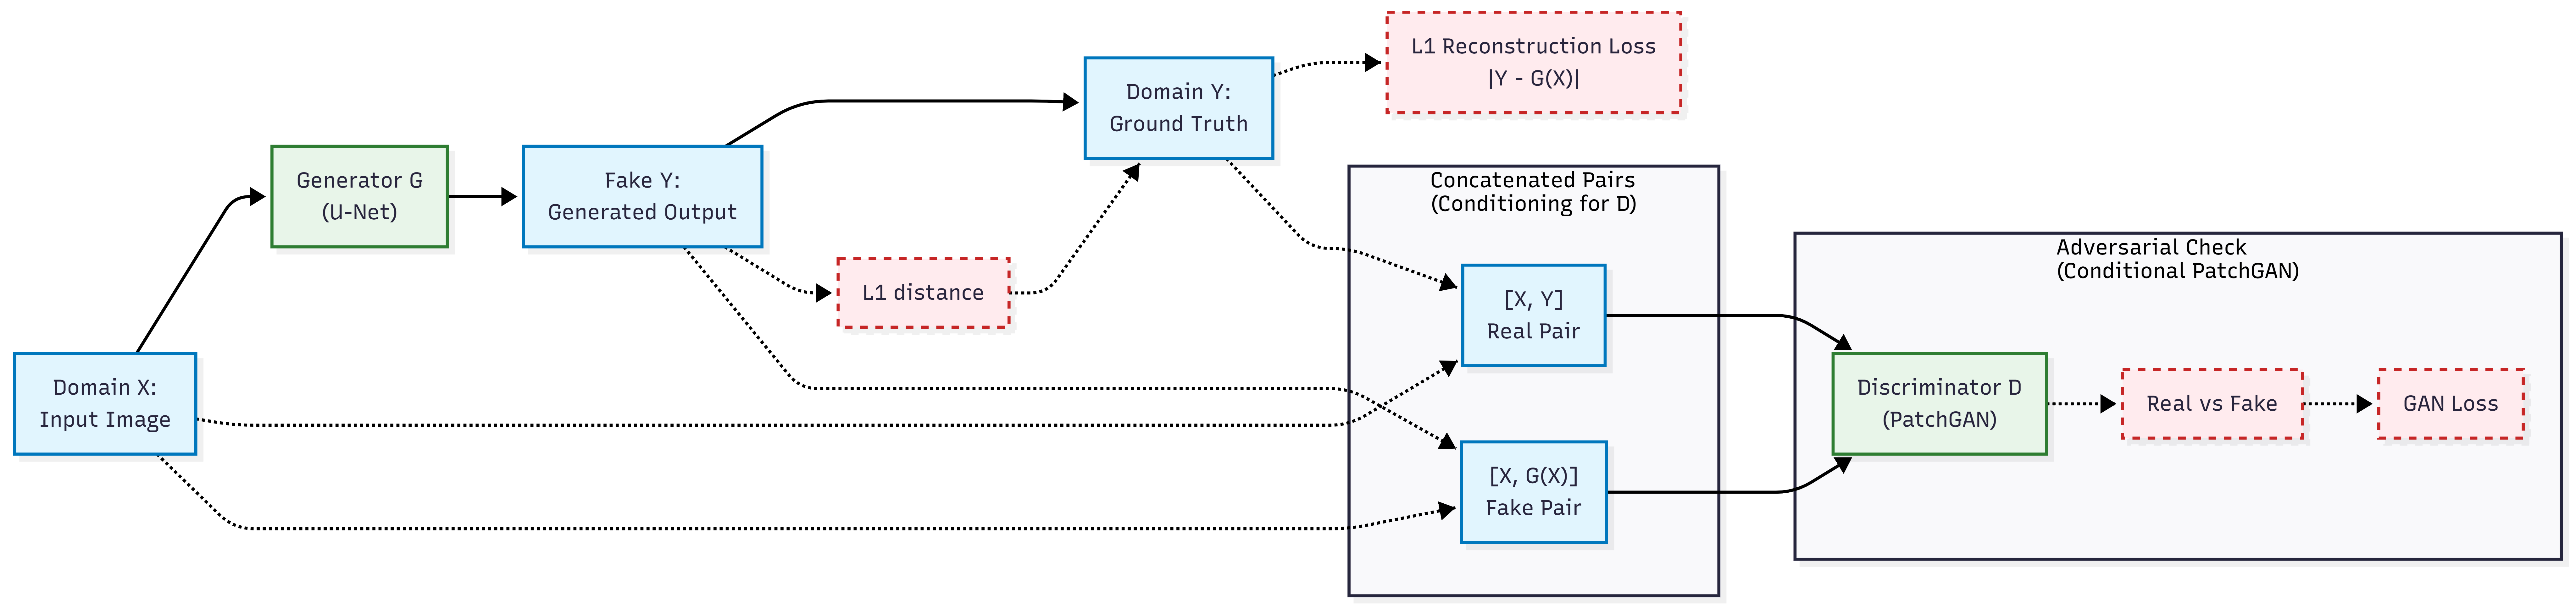
\includegraphics[width=\textwidth]{images/diagrams/pix2pix}
    \caption{Architecture of the Pix2Pix conditional GAN employed in the project. The generator translates simulated input maps into realistic radargrams efficiently using paired data supervision.}
    \label{fig:pix2pix_architecture}
\end{figure}

% \paragraph{Generator Architecture (U-Net with Skip Connections):}
\subsubsection{Generator Architecture: U-Net with Skip Connections}
\label{subsubsec:unet_generator}
The standard generator for the Pix2Pix model employs a modified \textbf{U-Net} architecture \cite{Ronneberger_2015}, a fully convolutional encoder-decoder network.
The complete topology of this network, including the downsampling bottleneck and the symmetric expansion path, was previously illustrated and detailed in Chapter~\ref{cha:preliminaries} (see Figure~\ref{fig:unet_architecture}).
The choice of U-Net is driven by the need to preserve low-level structural details (e.g., the precise depth of a subsurface interface) which are often lost in standard bottleneck architectures.

The \textbf{Encoder} is composed of 7 sequential blocks.
Each block typically consists of a Convolutional layer with a $4 \times 4$ kernel and stride 2 (performing spatial downsampling), followed by Instance Normalization and a LeakyReLU activation (slope 0.2).
This progressively compresses the $128 \times 128$ input into a latent feature representation of size $1 \times 1 \times 512$. 

The \textbf{Decoder} mirrors this structure using Transposed Convolutions (Deconvolutions) to upsample the feature maps back to the original resolution.
The critical innovation of the U-Net is the introduction of \textbf{Skip Connections}.
These connections concatenate the feature map from the $i$-th layer of the encoder directly to the $(n-i)$-th layer of the decoder.
Mathematically, if $E_i$ is the output of the encoder layer $i$, the input to the decoder layer $j$ becomes $[D_{j-1}, E_{n-j}]$.
This allows the unmodified high-frequency spatial information to flow directly to the output, bypassing the bottleneck.
For radar data, this is indispensable, ensuring that thin, sharp features like stratigraphic horizons are not blurred by the compression process.

\paragraph{Pix2Pix Loss Formulation:}
The objective of the Pix2Pix architecture combines a conditional adversarial loss with a traditional pixel-wise reconstruction loss, leveraging the availability of perfectly paired data.

\textbf{1. Conditional Adversarial Loss:}
Unlike a standard GAN that generates data from random noise, the conditional discriminator $D$ evaluates pairs of images: the input simulation $x_{sim}$ and either the real ground-truth radargram $x_{real}$ or the generated radargram $x_{gen} = G(x_{sim})$.
The generator $G$ tries to minimize this objective, while $D$ tries to maximize it:
$$ \mathcal{L}_{cGAN}(G, D) = \mathbb{E}_{x_{sim}, x_{real}}[\log D(x_{sim}, x_{real})] + \mathbb{E}_{x_{sim}}[\log(1 - D(x_{sim}, G(x_{sim})))] $$

\textbf{2. L1 Distance Loss:}
The adversarial loss alone is sufficient to generate sharp images, but it does not guarantee that the structural content matches the input.
To ensure the generated image captures the exact low-frequency structures (e.g., the correct depth of stratigraphic lines), an L1 regularization term is added.
It forces the generated image to be as close as possible to the ground truth at the pixel level:
$$ \mathcal{L}_{L1}(G) = \mathbb{E}_{x_{sim}, x_{real}}[\|x_{real} - G(x_{sim})\|_1] $$

The final objective for the Pix2Pix model is:
$$ \mathcal{L}_{Pix2Pix}(G, D) = \arg\min_G \max_D \mathcal{L}_{cGAN}(G, D) + \lambda \mathcal{L}_{L1}(G) $$
where $\lambda$ is a hyperparameter that controls the relative importance of the L1 term (typically $\lambda=100$, ensuring that structural fidelity dominates over pure adversarial realism).

\subsection{CycleGAN: Unpaired Translation}
The CycleGAN architecture \cite{Zhu_2017} represents a more sophisticated approach, removing the requirement for paired training data.
This is achieved by introducing two mapping functions: $G: X \rightarrow Y$ (Sim to Real) and $F: Y \rightarrow X$ (Real to Sim), and two discriminators $D_Y$ and $D_X$.

\begin{figure}[htbp]
    \centering
    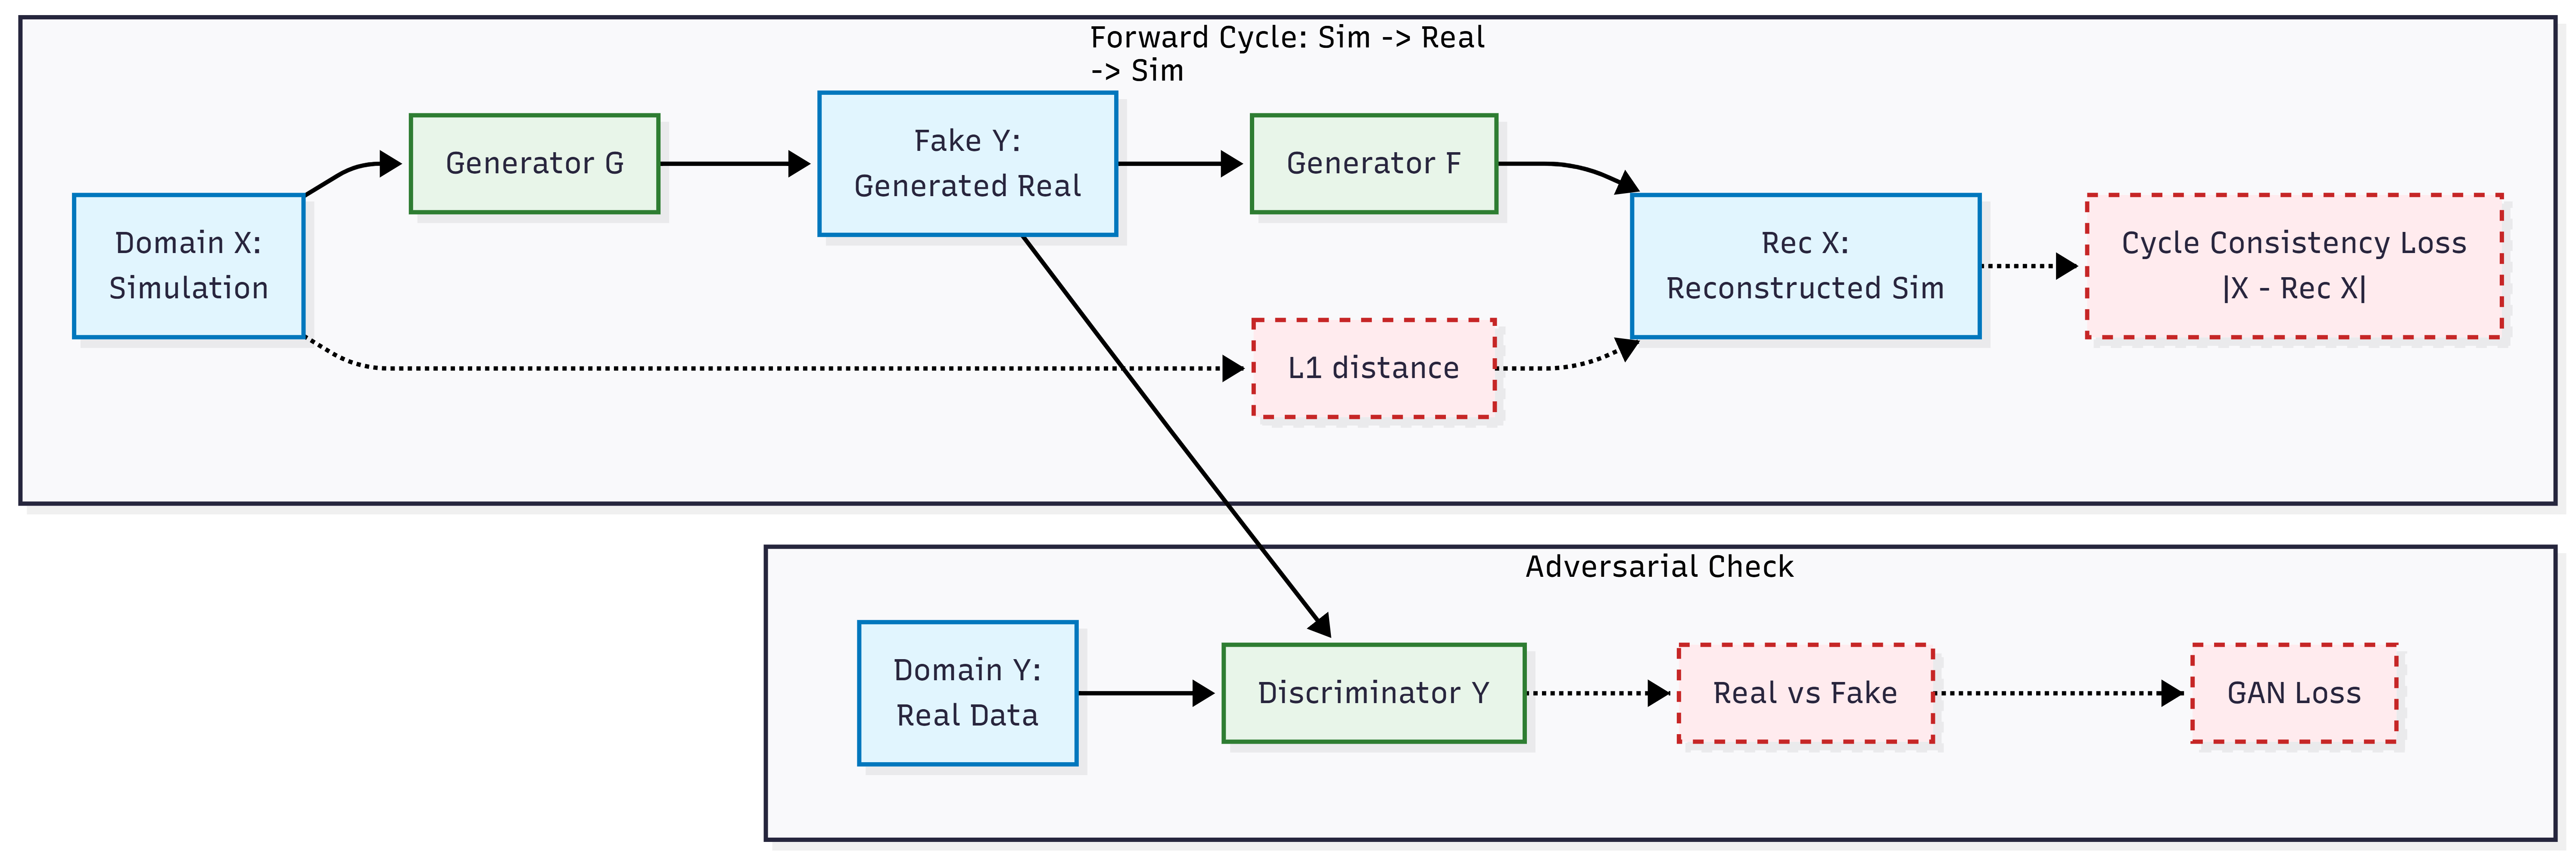
\includegraphics[width=\textwidth]{images/diagrams/cyclegan}
    \caption{Schematic of the CycleGAN architecture. The framework utilizes two generators and two discriminators to learn the mapping between simulated and real domains without paired examples, enforcing cycle consistency to preserve structural integrity.}
    \label{fig:cyclegan_architecture}
\end{figure}

\paragraph{Generator Architecture Variations:}
While CycleGAN can theoretically employ the same U-Net generator described in Section~\ref{subsubsec:unet_generator}, standard unpaired translation often favors a \textbf{ResNet-based} generator.
Unlike U-Net, which relies on direct skip connections between the encoder and decoder, ResNet transforms the features sequentially through residual blocks.
This prevents the network from aggressively copying the input via skip connections, avoiding artifacts in unpaired settings where the source and target are not perfectly aligned.
Thanks to the modularity of our framework, both U-Net and ResNet topologies are supported and can be dynamically instantiated.

\paragraph{CycleGAN Loss Formulation:}
The training objective of the CycleGAN architecture is a weighted sum of three distinct loss components, each serving a specific theoretical purpose to overcome the lack of paired supervision.

\textbf{1. Adversarial Loss:}
This standard GAN loss forces the generated images to be indistinguishable from real images.
For the mapping $G: \mathcal{X}_{sim} \rightarrow \mathcal{X}_{real}$, the objective is:
$$
\mathcal{L}_{GAN}(G, 
D_{real}, 
\mathcal{X}_{sim}, 
\mathcal{X}_{real})
=
\mathbb{E}_{x_{real}}
[\log D_{real}(x_{real})]
+
\mathbb{E}_{x_{sim}}
[\log(1 - D_{real}(G(x_{sim})))]
$$
Here, $G$ tries to minimize this objective (generate realistic samples), while $D_Y$ tries to maximize it (correctly classify real vs. fake).
A similar loss applies to the reverse mapping $F$.

\textbf{2. Cycle Consistency Loss:}
This is the core innovation of CycleGAN.
It enforces the constraint that translating a sample to the other domain and back should yield the original sample—effectively enforcing \textbf{Transitivity}.
If we translate a simulation $x_{sim}$ to a pseudo-real radargram $G(x_{sim})$, and then translate that back to a simulation using the reverse generator $F(G(x_{sim}))$, we should recover $x_{sim}$.
$$
\mathcal{L}_{cyc}(G, F)
=
\mathbb{E}_{x_{sim}}
\left[\|F(G(x_{sim})) - x_{sim}\|_1\right]
+
\mathbb{E}_{x_{real}}
\left[\|G(F(x_{real})) - x_{real}\|_1\right]
$$
This loss uses the L1 norm ($\|\cdot\|_1$) to penalize pixel-level differences.
Geologically, this is what preserves the stratigraphy: the model cannot simply generate a random realistic radar image; it must generate one that structurally corresponds to the input so that it can be translated back.

\textbf{3. Identity Loss:}
Often overlooked, the identity loss is critical for color and intensity preservation.
It states that if the generator $G$ (which converts Sim to Real) is fed an image that is \textit{already} from the Real domain ($x_{real}$), it should leave it unchanged:
$$
\mathcal{L}_{identity}(G, F)
=
\mathbb{E}_{x_{real}}
\left[\|G(x_{real}) - x_{real}\|_1\right]
+
\mathbb{E}_{x_{sim}}
\left[\|F(x_{sim}) - x_{sim}\|_1\right]
$$
In the context of radar, this prevents the generator from arbitrarily inverting the color palette or drifting the signal intensity.
It stabilizes the training by enforcing that the mapping is continuous near the target domain manifold.

The final full objective function is a weighted combination:
$$ \mathcal{L}(G, F, D_X, D_Y) = \mathcal{L}_{GAN}(G, D_Y, X, Y) + \mathcal{L}_{GAN}(F, D_X, Y, X) + \lambda \mathcal{L}_{cyc}(G, F) + 0.5 \lambda \mathcal{L}_{identity}(G, F) $$
where $\lambda$ controls the relative importance of cycle consistency (typically $\lambda=10$).

\subsection{Configuration-Driven Design}
To ensure rigorous experimental control and avoid "magic numbers" hardcoded in the source, the framework adopts a \textbf{Configuration-Driven Design}.
The entire experimental state is defined by declarative YAML configuration files (e.g., \texttt{config.yaml}).

This system allows for the strict separation of code (logic) and experiment (parameters).
Hyperparameters such as learning rates ($2 \times 10^{-4}$), architecture-specific loss weights ($\lambda_{cycle}=10.0$, $\lambda_{L1}=100.0$), batch sizes, and optimization strategies (Adam $\beta_1=0.5$) are injected at runtime.
This design explicitly supports the \enquote{Clean Code} principle, ensuring that running a new experiment (e.g., changing the cycle loss weight) requires no modification to the Python codebase, thereby eliminating the risk of introducing bugs during parameter tuning.
A summary of the baseline hyperparameter configurations used for both Pix2Pix and CycleGAN is presented in Table~\ref{tab:hyperparams}.

\begin{table}[htbp]
\centering
\caption{Summary of the Hyperparameter Configurations for Pix2Pix and CycleGAN Training}
\label{tab:hyperparams}
\begin{tabular}{lccc}
\hline
\textbf{Hyperparameter} & \textbf{Pix2Pix} & \textbf{CycleGAN} & \textbf{Description} \\ \hline
Input Resolution & $128 \times 128$ & $128 \times 128$ & Spatial dimensions of patches \\
Batch Size & 1 & 1 & Constraints due to Memory \\
Generator Learning Rate & $2 \times 10^{-5}$ & $2 \times 10^{-4}$ & Fixed \\
Discriminator Learning Rate & $1 \times 10^{-5}$ & $1 \times 10^{-4}$ & Fixed \\
Optimizer & Adam & Adam & Adaptive Moment Estimation \\
$\beta_1, \beta_2$ & $0.5, 0.999$ & $0.5, 0.999$ & Momentum terms \\
$\lambda_{L1}$ & $100.0$ & -- & Weight for L1 reconstruction loss \\
$\lambda_{cycle}$ & -- & $10.0$ & Weight for consistency loss \\
$\lambda_{identity}$ & -- & $5.0$ & Weight for identity loss \\
Epochs & 40 & 60 &Total training duration \\ \hline
\end{tabular}
\end{table}

\subsection{Micro-Architecture Definition}
To ensure stable training dynamics and high-fidelity texture synthesis, the abstract architectures described above were instantiated with a specific micro-architecture that departs in several aspects from standard CNN designs used for natural images.
In particular, the CycleGAN generators were implemented as 9-block ResNet networks with reflection padding and instance normalization, while the discriminators adopt a fully convolutional PatchGAN configuration with a finite receptive field over local patches.

\begin{figure}[htbp]
    \centering
    \begin{tikzpicture}[
        node distance=1.5cm and 1.5cm,
        box/.style={rectangle, draw, minimum width=2.8cm, minimum height=1.2cm, align=center, thick, rounded corners=2pt},
        arrow/.style={-{Stealth}, thick}
    ]
    
    % ---- RIGA SUPERIORE (Generazione) ----
    \node (sim) [align=center] {Simulated \\ Data ($x_{sim}$)};
    \node (gen) [box, right=of sim, fill=blue!10] {\textbf{Generator} ($G$) \\ \footnotesize{U-Net / ResNet}};
    \node (fake) [align=center, right=of gen] {Fake Radargram \\ ($x_{gen} = G(x)$)};
    
    % ---- RIGA INFERIORE (Discriminazione) ----
    % Posiziono il discriminatore esattamente sotto il fake radargram
    \node (disc) [box, below=1.2cm of fake, fill=red!10] {\textbf{Discriminator} ($D$) \\ \footnotesize{PatchGAN}};
    % I dati reali entrano da sinistra verso il discriminatore
    \node (real) [align=center, left=of disc] {Real \\ Radargram ($x_{real}$)};
    % L'output esce a destra
    \node (out) [align=center, right=of disc] {Real/Fake \\ Prediction};

    % ---- COLLEGAMENTI (Frecce) ----
    \draw [arrow] (sim) -- (gen);
    \draw [arrow] (gen) -- (fake);
    
    % Freccia che scende dal Fake al Discriminatore
    \draw [arrow] (fake) -- (disc);
    % Freccia dai dati reali al Discriminatore
    \draw [arrow] (real) -- (disc);
    
    \draw [arrow] (disc) -- (out);
    
    % ---- BOX TRATTEGGIATO OPZIONALE ----
    % Raggruppa la fase di discriminazione (Real, Fake, Disc, Out) per evidenziarla
    \draw[dashed, gray, thick] ([xshift=-0.5cm, yshift=0.3cm]real.west |- fake.north) rectangle ([xshift=0.3cm, yshift=-0.3cm]out.south east);
    
    \end{tikzpicture}
    \caption{Abstract schematic of the adversarial training framework. The Generator synthesizes realistic representations from simulated inputs, while the Discriminator evaluates both generated samples and real observations, outputting a probability score. The competing objectives of these two networks drive the optimization process.}
    \label{fig:gen_disc_scheme}
\end{figure}

\paragraph{Generator: 9-block ResNet with reflection padding}
The generator network $G$ follows a Johnson-style residual architecture and can be decomposed into three stages: downsampling, residual transformation, and upsampling.
The input is a single-channel radar patch $x \in \mathbb{R}^{1 \times 128 \times 128}$, already normalized to the range $[-1, 1]$ by the pre-processing pipeline described in Section \ref{sec:preprocessing_patching}.

\textbf{Downsampling.} The first stage consists of an initial $7 \times 7$ convolution with stride $1$ and reflection padding, followed by two strided convolutions ($3 \times 3$, stride $2$) that progressively reduce the spatial resolution while increasing the number of feature maps.
Concretely, the feature dimensionality evolves from $1 \times 128 \times 128$ to $64 \times 128 \times 128$, then to $128 \times 64 \times 64$, and finally to $256 \times 32 \times 32$.
Each block is followed by Instance Normalization (IN) and a ReLU activation, which together help to stabilize training across the highly heterogeneous dynamic range of radar echoes.

\textbf{Residual bottleneck.} The core transformation is implemented by a stack of 9 sequential residual blocks.
Each residual block $R_i$ applies the mapping
\[
y = F(x) + x,
\]
where $F(\cdot)$ is realized by two $3 \times 3$ convolutional layers with reflection padding, each followed by Instance Normalization and ReLU (except for the last activation, which is omitted to preserve the residual nature of the connection).
The use of reflection padding is critical in the radargram setting: zero padding would introduce artificial discontinuities at the patch borders (sharp transitions from valid signal to constant zeros), which the PatchGAN discriminator rapidly learns to classify as \enquote{fake}.
This mechanism typically manifests as grid-like artifacts at patch boundaries when tiling full radargrams.
Reflection padding, by mirroring the signal at the borders, preserves the continuity of stratigraphic horizons across patch edges and reduces such tiling artifacts.

\textbf{Upsampling.} The final stage restores the original spatial resolution through two transposed convolution layers with kernel size $3$ and stride $2$, which upsample the feature maps from $256 \times 32 \times 32$ back to $64 \times 128 \times 128$.
These are followed by a final $7 \times 7$ convolution with reflection padding and a $\tanh$ activation function, mapping the output back to the normalized range $[-1, 1]$.
This design ensures consistency with the Min-Max normalization adopted in Section \ref{subsec:minmax_normalization} and avoids mismatch between network outputs and input dynamic range.

Overall, this micro-architecture allows the generator to capture both local high-frequency patterns, such as speckle noise and small hyperbolic diffractions, and larger-scale structural features like continuous subsurface horizons, without sacrificing numerical stability.

\paragraph{Discriminator: PatchGAN with finite receptive field}
The discriminator $D$ is implemented as a Markovian PatchGAN, following the standard design of CycleGAN but adapted to the radargram patch size used in this work.
Unlike a conventional image-level discriminator that outputs a single scalar probability, PatchGAN maps the input image to a two-dimensional grid of real/fake scores, each associated with a local receptive field.

In the proposed architecture, $D$ is a 5-layer fully convolutional network with progressively increasing number of channels and stride $2$ in the first three layers.
For an input patch of size $128 \times 128$, the resulting receptive field of each output unit covers approximately a $34 \times 34$ pixel region in the original image.
In other words, each element of the discriminator output does not classify the entire image, but a local neighbourhood of fixed spatial extent.

Formally, let $D(x) \in \mathbb{R}^{H_D \times W_D}$ denote the discriminator response for an input $x \in \mathbb{R}^{1 \times 128 \times 128}$.
Each entry $D_{i,j}(x)$ corresponds to the discriminator's assessment of whether the $34 \times 34$ patch centered at position $(i,j)$ in the input domain is real or fake, based on the local texture statistics within its receptive field.
The adversarial loss is computed as the average over all these local decisions, enforcing realism at the patch level rather than only at the global image level.

This design choice is particularly well suited to SHARAD data.
Radargrams are characterized by stochastic speckle patterns and fine-scale textural variations that are poorly captured by purely global discriminators.
By constraining the discriminator to operate on local patches, PatchGAN explicitly encourages the generator to synthesize physically plausible high-frequency noise and clutter, while the cycle-consistency loss enforces the preservation of low-frequency global structure (e.g., the geometry of subsurface horizons).
The resulting adversarial game therefore decomposes the learning problem into complementary roles: the discriminator focuses on local realism, whereas the cycle-consistency and identity losses control the large-scale stratigraphic consistency of the translated radargrams.

